\section{Projet 9 — Le bandit manchot}

\subsection*{Objectif du jeu}
Simuler un bandit manchot (machines à sous) à 3 rouleaux et gérer le capital du joueur selon les combinaisons obtenues.


\subsection*{Règles du jeu}
\begin{itemize}
  \item 3 \textbf{rouleaux} de 11 figures (tableau 2D). Codes : \texttt{7, B, L, C} (sept, barre, citron, cerise).
  \item Le joueur commence avec \textbf{100 points} et mise 1 ou 3 points.
  \item Appui sur \texttt{J} : tirage aléatoire d’une figure par rouleau; affichage en ligne des trois codes.
  \item Le joueur gagne si une des combinaisons ci-dessous apparaît (\textbf{peu importe l'ordre}), sinon il perd sa mise ; le capital est mis à jour ; le joueur peut continuer (\texttt{O/N}).
\end{itemize}

\subsection*{Les rouleaux et les combinaisons}
\begin{center}
  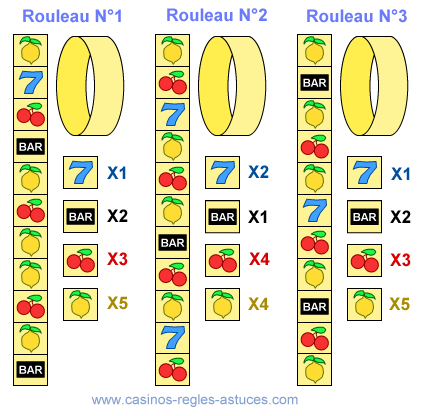
\includegraphics[width=0.5\textwidth]{sources/images/bandit_manchot_rouleaux.png}
\end{center}
Le gain est calculé à partir de la \textbf{mise} (1 ou 3 points) selon la combinaison obtenue, \textbf{peu importe l'ordre} des rouleaux :

\begin{center}
\begin{tabular}{|l|c|c|}
\hline
\textbf{Combinaison} & \textbf{Chances (environ)} & \textbf{Gain} \\ \hline
7 \quad 7 \quad 7 & 2 sur 1000 & mise $\times$ 500 \\ \hline
BAR \quad BAR \quad BAR & 3 sur 1000 & mise $\times$ 250 \\ \hline
Cerise \quad Cerise \quad Cerise & 3 sur 100 & mise $\times$ 25 \\ \hline
Citron \quad Citron \quad Citron & 7,5 sur 100 & mise $\times$ 10 \\ \hline
Citron \quad Citron \quad PAS Citron & 33 sur 100 & mise $\times$ 8 \\ \hline
Citron \quad PAS Citron \quad PAS Citron & 42 sur 100 & mise $\times$ 4 \\ \hline
\end{tabular}
\end{center}

Dans le programme : 7 est mémorisé par \texttt{'7'}, BAR par \texttt{'B'}, cerise par \texttt{'C'}, citron par \texttt{'L'}.

\textit{Conseils :} ranger les 3 figures tirées dans un tableau ; en mode test, vous pouvez modifier les rouleaux pour favoriser une combinaison.

\subsection*{Cahier des charges}
\begin{UPSTICahierDesCharges}{1}
\begin{itemize}
  \item Initialiser les \textbf{3 rouleaux} (tableau 3×11) et afficher leur contenu pour vérification.
  \item Tirer et afficher \textbf{une figure par rouleau} (codes).
  \item Mettre à jour le capital selon résultat simple (ex.\,égalité des 3).
\end{itemize}
\end{UPSTICahierDesCharges}

\begin{UPSTICahierDesCharges}{2}
\begin{itemize}
  \item Implémenter les \textbf{mises} (1 ou 3), détailler les combinaisons gagnantes/perdantes.
  \item Si aucune combinaison n'apparaît, le joueur peut \textbf{rejouer} un ou plusieurs rouleaux (ex.\,saisie \texttt{23} pour rejouer les rouleaux 2 et 3, puis \texttt{J}) ; il perd alors 1 point (ou 3 selon la mise de départ). Et ainsi de suite jusqu'à obtenir une combinaison ou ne plus avoir de points.
  \item Récapitulatif clair de fin.
\end{itemize}
\end{UPSTICahierDesCharges}

\begin{UPSTICahierDesCharges}{3}
\begin{itemize}
  \item Présentation et rejouabilité; options de test (rouleaux biaisés).
  \item Structuration en fonctions (tirage, calcul gain, affichage).
  \item Robustesse des saisies.
\end{itemize}
\end{UPSTICahierDesCharges}

